% Chapter 3

\chapter{Problem} % Main chapter title

\label{Chapter3} % For referencing the chapter elsewhere, use \ref{Chapter1} 

\lhead{Chapter 3. \emph{Problem}} % This is for the header on each page - perhaps a shortened title

\section{Ocelot Overview}

\subsection{Main Design Principles}

Ocelot is a hardware-oblivious parallel database engine. The motivation for opting for \textit{hardware-oblivious} design which is the opposite of the \textit{hardware-aware} design stems from the ongoing shift to heterogeneous architectures that feature various computing devices of possibly different architectures on a single platform. Ocelot fulfills its hardware-oblivious design goal by abstracting away the details of the hardware components at the design time. As discussed in \citep[p. 710]{heimel_hardware-oblivious_2013}, hardware abstraction is needed to deal with following problems of hardware-aware design.

\begin{itemize}
\item{Database vendors focus on only few architectures for hardware specific fine-tuning of the database engine in order to limit the development and maintenance costs.}
\item{It is not possible to use existing operator implementations for a new architecture aimed to be supported. This simply requires reimplementation of the whole set of operators.}
\item{With each additional architecture to be supported, database vendors have to extend their expertise area on a particular hardware beyond their core competences.
}
\end{itemize}

With the hardware details are abstracted away, database-engine developers can use a high-level language to program database operators in a main codebase repository. Then, the compilers that are provided by the hardware vendors compile the operator algorithms available in the main codebase into the binary code. In Ocelot, the high-level programming of the operators is done using the \textit{Kernel Programming Model}. According to \citep[pp. 710-711]{heimel_hardware-oblivious_2013}, in this model, programs consist of a number of kernels each of which define an operation on single element of the input data. These operations then operate on the input in a \textit{lock-free} fashion. Although, by its design, this kernelized programming approach seems to be specifically tailored for GPUs that feature a massive parallelism, they can run on single-core architecture by simply running the kernels sequentially on the input thanks to their highly abstract definition. More examples of the how the kernelized programs are executed in different architectures are presented in \citep[p. 711]{heimel_hardware-oblivious_2013}.

\subsection{Self-Adaptivity}

Kernel Programming model makes it possible to port the programs to different architectures. This is why, it is the main essence of hardware obliviousness. However, the portability is not the only concern. The portable operator programs implemented should also run efficiently on the ported architecture. In order to achieve this efficiency, hardware-dependent optimizations should be done. However, It is not possible to write the operator code tailored for an architecture as it would then break the hardware-oblivious design principle. In order to carry out hardware-dependent optimizations without being hardware-aware, Ocelot features self-adaptivity. Self-adaptivity is achieved in two steps. First, a large number of variants of the operator algorithms either at the design time or dynamically at the run time are prepared. Then, Ocelot attempts to pick the most performant one on the fly. The optimal operator algorithm variant given the features such as input size, etc can be different for different computing devices as the capabilities of different kind of devices are naturally different. Furthermore, the optimal operator variant for a given operator task scenario can also differ within the same kinds of device. Even for the models from the same vendor sharing the same architecture, the optimal variant could be potentially different. Considering the exploding number of combinations of different models of the different hardware can be present together on a platform, picking the most optimal operator variant given the input characteristics (features) for each device at the Ocelot's disposal is a challenging task. Following, the details of this decision-making process is discussed.

Ocelot separates the device selection routine and the algorithm selection routine. Device selection logic considers the performance statistics of the devices for the current operator with given features as well as the other factors such as the current load of the available devices and the transfer times between devices. Once a device for the current operator to be offloaded to is selected, algorithm selection logic decides on the algorithm to be used to obtain the output for the operator. 

The algorithm selection logic is complex. It is based on the runtime predictions for all the choices of algorithms available for the current operator. However, each algorithm is implemented by a big number of kernelized variants. Moreover, for each algorithm, an \textit{active set} of variants that implements the algorithm are maintained. A cost model associated with each variant in the active set is also maintained. When the runtime prediction for an algorithm is requested in order to choose the most performant algorithm for the given input, the lowest of the predictions of these cost models are returned. After an algorithm is chosen, all the variants in the active set is executed and runtime measurements of each of them are recorded. These measurements are used to update the cost models. Initially when the database in its \textit{cold start} phase and not have adapted itself yet to the underlying hardware, the cost models for the active set are empty predictive models hence they do not make good runtime predictions. As more queries are passed to the database engine and more operators are executed, the cost models for the active set variants of the chosen algorithms become mature predictive models and starts delivering good runtime estimations when the algorithm selection logic requests the runtime predictions before choosing an algorithm. This means runtime predictions of a certain algorithm for an operator is reliable only after the algorithm is selected a number of times. This represents a \textit{multi-armed bandit} problem in which there is a trade-off between \textit{exploitation} and \textit{exploration} \citep[p. 618]{heimel_demonstrating_2014}. In Ocelot, decaying $\epsilon$-greedy approach is employed to balance exploitation of the cost models learned for the variants of the algorithm options for an operator to pick the most performant algorithm and the exploration of the performance characteristics of the available algorithms to improve cost models of the underlying active set of variants of them. With $\epsilon$-greedy approach employed, the algorithm selection routine, with probability of $1-\epsilon$, picks the \textit{supposedly} most performant algorithm indicated by the minimum of the estimated runtimes of the active set variants of each algorithm. With probability of $\epsilon$, algorithm selection routine picks a random algorithm other than the supposed most performant one.

The active set of the variants of an operator algorithm is a dynamic set and it is dynamically updated on the fly. When there is a variant in the active set which performs badly in comparison to the other ones, it is replaced by another variant from the library of variants each algorithm has. Alternatively, a variant could be just dropped without an alternative variant taking its place. This dynamically evolving active set is expected to converge to a state with a single-element active set with the only variant that is the optimal one among the variants defined in the variant library. This variant is expected to as close as possible to the \textit{hand-tuned} implementation of the corresponding algorithm of the variant in a hardware-aware database.

How the device selection and algorithm selection work together to realize self-adaptivity goal is sketched in Figure \ref{fig:Ocelot}.

\begin{figure}[htbp]
  \centering
    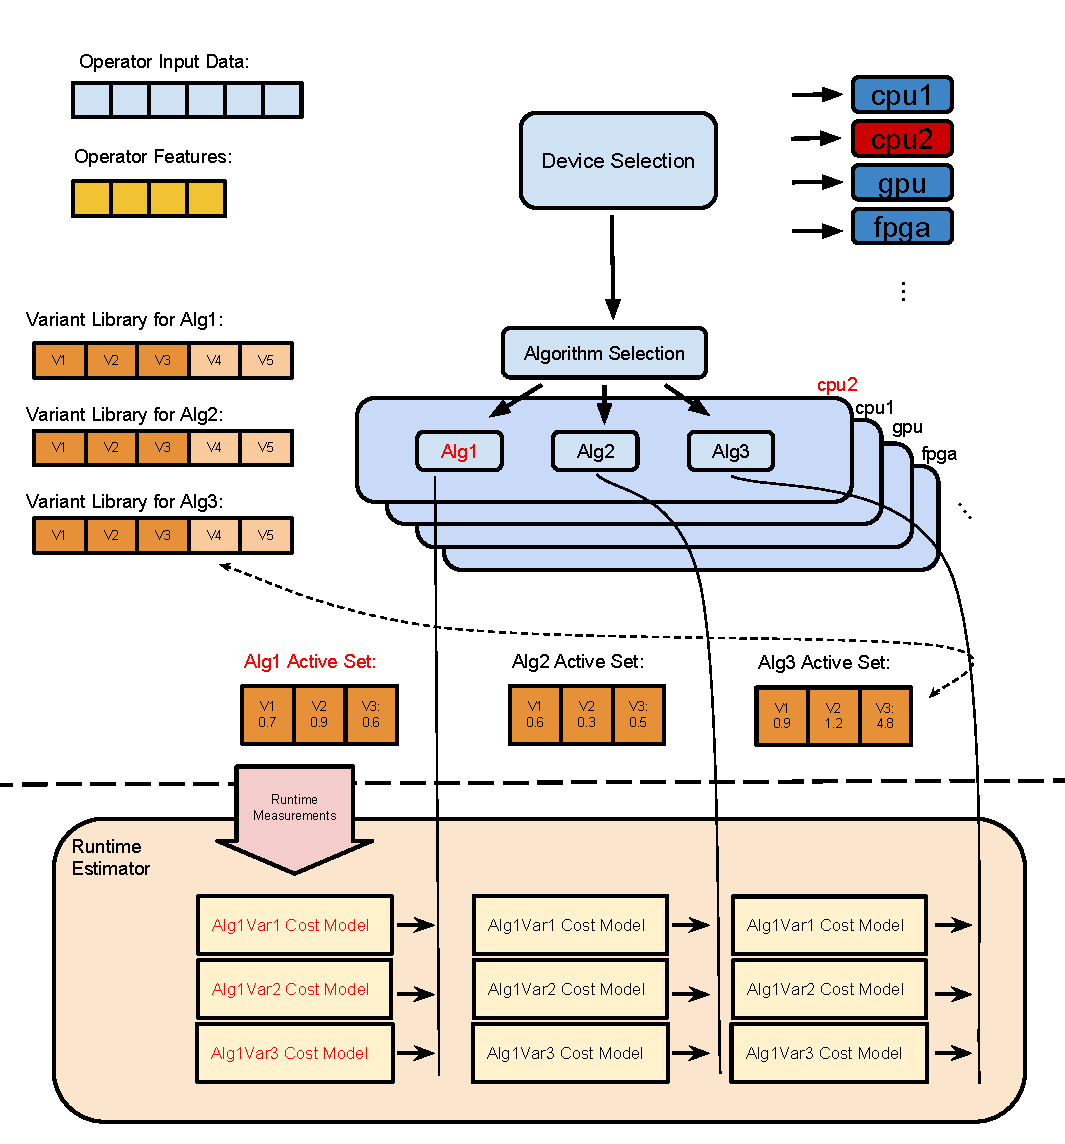
\includegraphics[width=\linewidth]{./Figures/Ocelot.pdf}
  \caption{Overview of the device and algorithm selection in Ocelot. Note that the numbers written in the boxes that represent the active algorithm variant set denote the average runtime of the corresponding variant.}
  \label{fig:Ocelot}
\end{figure}

\section{Learning Problem}

\subsection{Correspondence to Data Stream Learning}

In Ocelot, the task of building and updating cost models is abstracted away from the algorithm selection routine. The space above the dotted line in \ref{fig:Ocelot} has an abstract view of the bottom part which depicts the \textit{Runtime Predictor}. Algorithm selection routine is provided with an interface of two functionalities namely update and predict. Whenever an algorithm selection is needed, the algorithm selection routine requests runtime predictions for the algorithms and after the execution of the selected algorithm on the selected device, it updates the runtime estimator with the measured runtime data. 

Runtime estimator module is totally blind to decision-making layers such as algorithm selection and device selection. It can be thought of a utility component with a global state. Within the Runtime Estimator, for each  existing algorithm-variant-hardware combination, there is a corresponding cost-model. This cost model is required to be refined with new measurements and predict the actual cost of its variant accurately as explained in the previous section. Obviously, this is a machine learning problem where an updatable predictive model is needed for fulfilling the requirements of the runtime estimator.

The learning scenario with the runtime estimator module represents the characteristics of stream learning described in \ref{section:data_stream_learning}. Initially empty predictive models (cost models) are first used to make a prediction (runtime estimate) for a feature set of a predefined size (characteristics of the current input) then, they are provided with a real number (the noisy measurement of the runtime) to refine the predictive model. These two operations of predict and update occur repeatedly one after another potentially infinite number of times. \ref{fig:Ocelot2} pictures this particular learning scenario.

\begin{figure}[htbp]
  \centering
    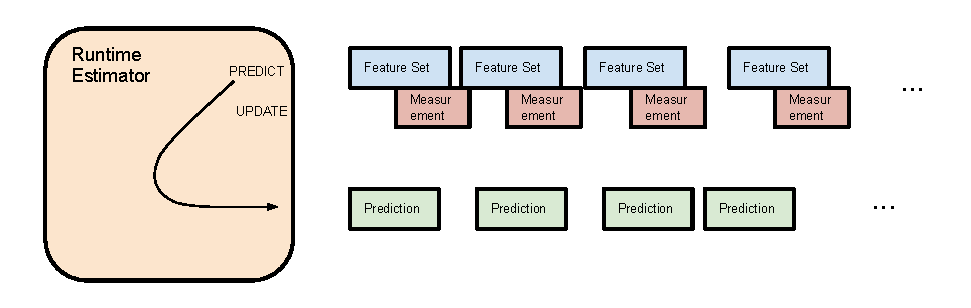
\includegraphics[width=\linewidth]{./Figures/Ocelot2.pdf}
  \caption{Runtime Predictor is visualized as a stream learner. Note that the irregular spacing between the arriving items as well as between the predictions illustrates that the frequency of runtime predictions are requested by the algorithm selection logic of the Ocelot is variable}
  \label{fig:Ocelot2}
\end{figure}

Data stream in the runtime estimation scenario can be seen as an array of feature sets that describe the characteristics of the inputs to the operators and the measurements. For the sake of adapting the machine learning jargon, the feature sets and the measurements are referred to as \textit{data points} and the \textit{targets} respectively in the rest of the thesis. 

The process that generates the data points and their targets in this scenario is very complex and it depends myriad of things. Among these dependencies of the data generation process, the Ocelot-relevant ones are the performance of the active set variants for an algorithm and the behavior of the algorithm variant replacement logic. Primarily, the former affect the runtimes observed. However, the latter dramatically and abruptly change the measured runtimes. Although, it is stated above that there is a cost model for each possible variant-algorithm-device combination, this is an oversimplification. Since the Runtime Estimator is not aware of the algorithm variant substitutions, it keeps a cost-model for the variant that sits in a certain place in the active set. The implication of this is important in terms of the produced runtime measurement data which is used to update the cost models. When an algorithm variant is replaced, the cost model maintained for the replaced variant \textbf{immediately} becomes obsolete. Thus, through the update calls from the algorithm selection logic, it is expected to become an accurate performance estimator of the new variant substituted in. This corresponds to \textit{learning from non-stationary streams} scenario as discussed in \ref{subsection:2.4.1}. 

Data horizon for this online learning scenario is very close as new measurement after concept drifts are needed to be incorporated into the cost models immediately whereas the data horizon once the cost models become good predictors of the runtimes is infinitely far meaning the new measurements cannot be used to improve the accuracy of the cost models more. Similarly, the data obsolescence time is zero after concept drifts as the cost model that becomes obsolete is built with old data points. However, once the learning algorithm stabilizes and the cost model again become a good predictor of the runtime measurements, the effect of old data points on the predictive models do not need to be removed meaning that data obsolescence time is infinite.

Data generation process also depends on more general things other than the internals of Ocelot. Among these are the potential measurement error, potentially varying performance of the hardware components, number of context switches scheduled by the scheduler of the Operating System running on the platform that Ocelot is deployed. As a result of these, it is not possible to get noise-free runtime measurements for operator algorithm variant runtimes. The noise is assumed to be feature and operator independent (homoscedastic noise). 

\subsection{Required Properties of the Learning Model}

Having described the learning problem posed by the Ocelot's runtime estimation needs in the previous section, in this section, the requirements that the learning algorithm to be employed should meet are discussed.

In the following, these requirements are listed and described.

\begin{itemize}
\label{list:restimator_requirements}

\item \textbf{High accuracy:} The predictive models used as cost models to predict runtimes should make estimations with high accuracy so that the algorithm selection and the device selection routines can make good decisions.
\item \textbf{Robust to Abrupt Concept Drifts:} Whenever the algorithm variant substitution mechanism fires and replaces a variant with a new one from the variant library, the runtime measurements given the features potentially change as explained in the previous chapter. This change can be seen as a concept drift. This is because, the most important factor that affects the distribution of the target values given the features is the performance of the algorithm variant and once the variant itself is different, the underlying data distribution of the features and the targets unavoidably changes. However, when some number of the feature-target pairs are sampled from the old and new underlying distributions, the functions that can fit these samples are expected to have the same growth rate. This is because, although the variants for the same algorithm have different implementations of the same algorithm, since they implement the same logic described in the pseudocode of the algorithm, the performance characteristics of the variants are expected to be similar. 
The learning algorithm used for building predictive models which are used as cost models in the Ocelot context should be robust to abovementioned concept changes. However, this does not impose any kind of restrictions on the update frequency of the predictive model on the contrary to how it is illustrated by the red boxes in \ref{fig:Ocelot2} where the cost model is pictured to be updated after every single runtime estimation made and also how it is implies by the online prediction protocol presented in the pseudocode \ref{alg:opp}. Online learning algorithm has two different mechanism in order to deal with abrupt concept drifts. First, it can either update the predictive model with every single new runtime measurement and never worry about the detection of concept drifts. Second, it can implement a drift detection method and update the model incrementally with the new runtime measurements until an accurate predictive model is obtained only after a concept drift is detected or during the \textit{cold start} phase when the predictive models are empty.
\item \textbf{Robust to Measurement Noise:} As mentioned in the previous section, the measured runtimes that is used to update the predictive models are not noise-free. This requires the learning algorithm to be able to learn from the measurement data contaminated by homoscedastic noise. 
\item \textbf{Provide bounds for estimates:} The sophisticated algorithm selection logic of Ocelot requires more than just a point prediction of the runtime. Under some conditions, which are not covered and considered to be in the scope of this thesis work, it bases its algorithm-selection decision on the potentially minimum or potentially maximum runtime of the algorithm variants estimated for given features. This requirement makes sense when the difficulty of making point predictions with the noisy training data is considered. In short, the learning algorithm should produce estimations given the features that consist of three elements namely lower prediction bound, point prediction and upper prediction bound. The interval marked by the upper and lower prediction bounds should cover the observed runtimes with a high confidence level.
\item \textbf{Efficiency:} Although the amount of time between individual predictions requested by the algorithm selection logic for an operator algorithm is not fixed and it depends on many factors such as the distribution of the different operators that make up the queries that are passed to Ocelot and the device selected by the device selection logic, it is hard to set a minimum required datarate that runtime estimator module can handle. Generally speaking, runtime estimator module should ideally run fast enough so that algorithm selection logic never has to delay its decision. It is hard to foresee the time-efficiency requirements without knowing the maximum call frequency the algorithm selection routine\footnote{During the period this thesis work was being carried out, no such information was available}. Nevertheless, as an initial time-efficiency target to be achieved, the delay that runtime estimator module causes per runtime estimation together with the update operation with the observed runtime should not exceed $1$ ms.

\end{itemize}

% In the following Chapter, the online learning approaches that can meet the above requirements in theory are discussed.

% The reason for the discontinuity is that in real-life operator runtime estimation scenario, the operator cost models to be learned are most likely to be actually discontinuous functions. The reason for the concept drift choice is that as explained in [ref], Ocelot is expected to rep running operator algorithm variants resulting in the cost model to be learned dynamically change another one which can be best mocked by an abrupt change of the function that the data set 